\section{Mở rộng: bộ dữ liệu khác, tăng cường dữ liệu, CNN và trình khám phá thực thi}
\label{sec:extensions}

Phần này dùng \emph{cùng mã, cùng giao thức và cùng bộ đánh giá} như các mục trước. Mọi bảng và hình được sinh từ các tệp trong \texttt{results/}; các thí nghiệm được chạy lại bằng dòng lệnh (README). Các kết luận chỉ có giá trị cho các bộ dữ liệu và cấu hình đã đo.

\subsection{Fashion-MNIST và EMNIST Digits}
\label{sec:datasets}
Cả hai bộ đều là ảnh xám $28\times28$ với $10$ lớp nên dùng lại nguyên pipeline. \textbf{Fashion-MNIST} (áo thun, quần, áo len, \ldots, giày cao cổ) có $60\,000$ ảnh train và $10\,000$ ảnh test chính thức. \textbf{EMNIST Digits} có $240\,000$ ảnh train và $40\,000$ ảnh test chính thức; chúng tôi lấy một tập con phân tầng $60\,000$ ảnh từ phần train, chia $50\,000/10\,000$ thành train/validation (cùng kích thước như MNIST để thời gian có thể so sánh), giữ nguyên $40\,000$ ảnh test, và lật/xoay ảnh về chiều đứng như MNIST. Mỗi bộ có phép chia riêng, thống kê chuẩn hóa riêng (chỉ từ train của bộ đó), siêu tham số chọn riêng trên validation của bộ đó bằng quét \emph{rút gọn} (ít giá trị hơn so với MNIST để vừa ngân sách thời gian), và kết quả được báo cáo \emph{tách biệt} với MNIST.

Định nghĩa lớp khác nhau: MNIST và EMNIST Digits đều gán nhãn $0$--$9$ cho chữ số, còn Fashion-MNIST gán $10$ loại quần áo cho cùng các chỉ số $0$--$9$. Vì vậy một mô hình huấn luyện trên một bộ \emph{không} được đánh giá trên bộ có định nghĩa lớp khác: chương trình từ chối phép đó. Phép kiểm tra chéo duy nhất hợp lệ là MNIST $\to$ EMNIST Digits, và nó chỉ được báo cáo cho đúng mô hình huấn luyện trên MNIST, tách khỏi mô hình huấn luyện trên EMNIST. Trang web cũng ghi rõ bộ dữ liệu, tên lớp và mô hình đang dùng ở mọi nơi.

\begin{table}[tbp]\centering\small
\begin{tabular}{lrrr}
\toprule
Mô hình & MNIST & Fashion-MNIST & EMNIST Digits \\
\midrule
Gaussian NB & 81.32 / 81.16 & 67.27 / 66.03 & 80.03 / 80.13 \\
Softmax regression & 92.52 / 92.42 & 84.27 / 84.18 & 93.81 / 93.81 \\
MLP & 98.24 / 98.23 & 88.59 / 88.55 & 98.36 / 98.36 \\
AdaBoost-SAMME & 97.60 / 97.58 & 84.74 / 84.88 & 97.38 / 97.38 \\
CNN & 98.80 / 98.79 & 88.49 / 88.48 & 98.64 / 98.64 \\
\bottomrule
\end{tabular}
\caption{Accuracy / macro-F1 trên tập test (\%) của từng bộ dữ liệu; mỗi bộ dữ liệu có phép chia train/validation/test riêng, siêu tham số chọn riêng trên validation của bộ đó (quét rút gọn cho Fashion-MNIST và EMNIST Digits). Không so sánh chéo giữa các bộ dữ liệu.}
\label{tab:datasets}
\end{table}


Bảng~\ref{tab:datasets} cho thấy thứ hạng thay đổi theo bộ dữ liệu: các mô hình có cấu trúc (MLP, CNN) vượt xa Naïve Bayes trên Fashion-MNIST, (một cách giải thích hợp lý, chưa được kiểm chứng riêng, là giả thiết các pixel độc lập có điều kiện kém phù hợp hơn với ảnh quần áo), và khoảng cách giữa các mô hình thu hẹp hay nới rộng tùy bộ dữ liệu. Vì siêu tham số của hai bộ mới được chọn bằng quét rút gọn một seed, chênh lệch nhỏ giữa MLP và CNN ở đó không đủ để kết luận mô hình nào tốt hơn. Với EMNIST Digits chúng tôi không chạy baseline scikit-learn (tốn thời gian và không cần cho câu hỏi ở đây), nên bộ này chỉ có kết quả của các bản tự cài đặt.

\textbf{Kiểm tra chéo MNIST $\to$ EMNIST Digits.} Đây là phép duy nhất hợp lệ về định nghĩa lớp (Bảng~\ref{tab:cross-eval}). Mô hình huấn luyện trên MNIST tụt mạnh khi gặp EMNIST (Naïve Bayes xuống dưới $50\%$), trong khi mô hình huấn luyện trên chính EMNIST đạt $80.0\%$ (Naïve Bayes) và $98.6\%$ (CNN); CNN giữ được nhiều nhất. Chúng tôi chưa tách riêng nguyên nhân; một giả thuyết hợp lý là kiểu chữ, kích thước và cách căn giữa của hai bộ khác nhau, và các mô hình có cấu trúc không gian chịu được dịch chuyển tốt hơn. Kết quả này chỉ nói về hai bộ dữ liệu này và không phải bằng chứng về khả năng tổng quát hoá sang chữ viết tay nói chung.

\IfFileExists{generated/cross_eval.tex}{\begin{table}[H]\centering\small
\begin{tabular}{lrr}
\toprule
Mô hình & Huấn luyện trên MNIST & Huấn luyện trên EMNIST Digits \\
\midrule
Gaussian NB & 49.80 & 80.03 \\
Softmax regression & 53.59 & 93.81 \\
MLP & 76.70 & 98.36 \\
CNN & 92.15 & 98.64 \\
AdaBoost-SAMME & 73.69 & 97.38 \\
\bottomrule
\end{tabular}
\caption{Accuracy (\%) trên $40\,000$ ảnh test của EMNIST Digits. Cột giữa là mô hình huấn luyện trên MNIST (dùng hằng số chuẩn hóa của MNIST) đánh giá trực tiếp; cột phải là mô hình huấn luyện trên EMNIST Digits. Đây là hai mô hình khác nhau.}
\label{tab:cross-eval}
\end{table}
}{}

\subsection{Tăng cường dữ liệu: thí nghiệm có đối chứng}
\label{sec:augmentation}
Năm phép biến đổi (Hình~\ref{fig:aug-examples}), chỉ áp dụng cho tập train, nhãn không đổi: \emph{xoay} đều trong $[-15^\circ,15^\circ]$; \emph{dịch} đều trong $[-2,2]$ pixel theo mỗi trục; \emph{co giãn} đều trong $[0.9,1.1]$; \emph{nhiễu Gauss} $\sigma=0.1$ trên thang $[0,1]$; \emph{nhiễu muối tiêu} với $2\%$ pixel. Các phép hình học được gộp thành một phép affine duy nhất cho mỗi ảnh (nội suy song tuyến tính); đây là biến đổi dữ liệu chứ không phải thành phần của mô hình.

Bố trí thí nghiệm: giữ nguyên siêu tham số, seed và quy tắc dừng sớm; chỉ đổi tập huấn luyện. Điều kiện $c$ thêm một bản sao biến đổi của mỗi ảnh train ($100\,000$ ảnh, gấp đôi điều kiện gốc), nên có \emph{hai yếu tố trộn lẫn}: loại biến đổi và việc có thêm dữ liệu/bước cập nhật. Có tám điều kiện (gốc; từng phép riêng lẻ; nhóm hình học; cả năm), mỗi điều kiện chạy nhiều seed và so sánh \emph{ghép cặp theo seed}. Điều kiện được chọn \emph{chỉ} theo validation accuracy trung bình; test chỉ được báo cáo. Độ bền được đo thêm bằng ảnh test biến đổi cố định (seed 999) ở mức \emph{mạnh hơn} lúc huấn luyện (xoay $20^\circ$, dịch 3 pixel, co giãn $0.8$--$1.2$, $\sigma=0.2$, $4\%$ muối tiêu), dùng chung cho mọi mô hình và chỉ để báo cáo.

\begin{figure}[H]\centering
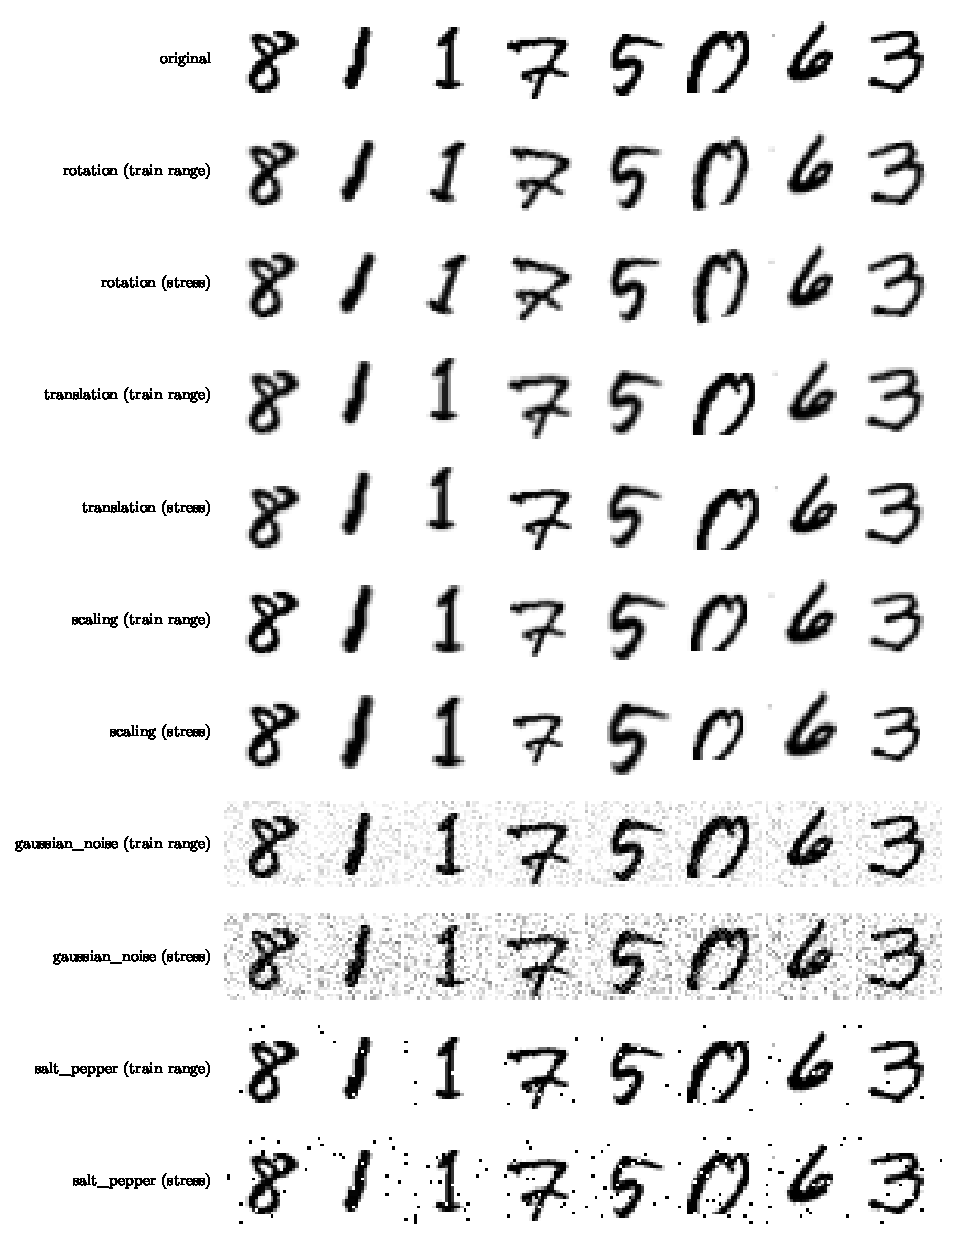
\includegraphics[width=0.7\textwidth]{../results/figures/augmentation_examples.pdf}
\caption{Ảnh gốc và từng phép biến đổi ở mức huấn luyện và mức kiểm tra độ bền (cùng các ảnh nguồn).}
\label{fig:aug-examples}
\end{figure}

\begin{table}[H]\centering\scriptsize
\setlength{\tabcolsep}{3pt}
\begin{tabular}{lrrrrrrrrr}
\toprule
 & & \multicolumn{2}{c}{Validation} & Test & \multicolumn{5}{c}{Test sau nhiễu (\%)} \\
\cmidrule(lr){3-4}\cmidrule(lr){6-10}
Điều kiện & Số mẫu & Acc (\%) & $\Delta$ so với gốc & Acc (\%) & Xoay & Dịch & Co giãn & Gauss & Muối tiêu \\
\midrule
Không tăng cường & 50\,000 & 97.88 $\pm$ 0.42 & +0.00 $\pm$ 0.00 & 98.02 & 95.8 & 72.1 & 96.5 & 97.1 & 97.4 \\
Xoay & 100\,000 & 98.45 $\pm$ 0.06 & +0.57 $\pm$ 0.47 & 98.48 & 97.6 & 75.9 & 97.1 & 97.6 & 98.0 \\
Dịch chuyển & 100\,000 & 98.43 $\pm$ 0.30 & +0.54 $\pm$ 0.55 & 98.41 & 96.6 & 94.5 & 97.5 & 97.6 & 97.8 \\
Co giãn & 100\,000 & 98.30 $\pm$ 0.10 & +0.42 $\pm$ 0.45 & 98.33 & 96.3 & 75.7 & 97.5 & 97.4 & 97.7 \\
Nhiễu Gauss & 100\,000 & 98.27 $\pm$ 0.01 & +0.38 $\pm$ 0.42 & 98.35 & 96.3 & 74.4 & 96.9 & 97.7 & 97.9 \\
Nhiễu muối tiêu & 100\,000 & 98.25 $\pm$ 0.04 & +0.37 $\pm$ 0.40 & 98.32 & 96.3 & 74.1 & 96.7 & 97.5 & 97.9 \\
Hình học (xoay, dịch, co giãn) & 100\,000 & 98.19 $\pm$ 0.21 & +0.31 $\pm$ 0.33 & 98.24 & 97.1 & 94.3 & 97.4 & 97.1 & 97.6 \\
Cả năm phép & 100\,000 & 97.98 $\pm$ 0.03 & +0.09 $\pm$ 0.40 & 98.11 & 96.8 & 93.7 & 97.2 & 97.3 & 97.5 \\
\bottomrule
\end{tabular}
\caption{MLP với cấu hình đã chọn, huấn luyện lại với 3 seed (42, 43, 44) cho mỗi điều kiện; $\Delta$ là hiệu validation accuracy so với điều kiện gốc \emph{cùng seed} (trung bình $\pm$ độ lệch chuẩn mẫu). 1 bản sao biến đổi cho mỗi ảnh train; điều kiện được chọn chỉ theo validation (\texttt{rotation}). Các cột ``Test sau nhiễu'' đo độ bền trên tập test bị biến đổi ở mức mạnh hơn mức huấn luyện, chỉ để báo cáo.}
\label{tab:augmentation-mlp}
\end{table}

\begin{figure}[H]\centering
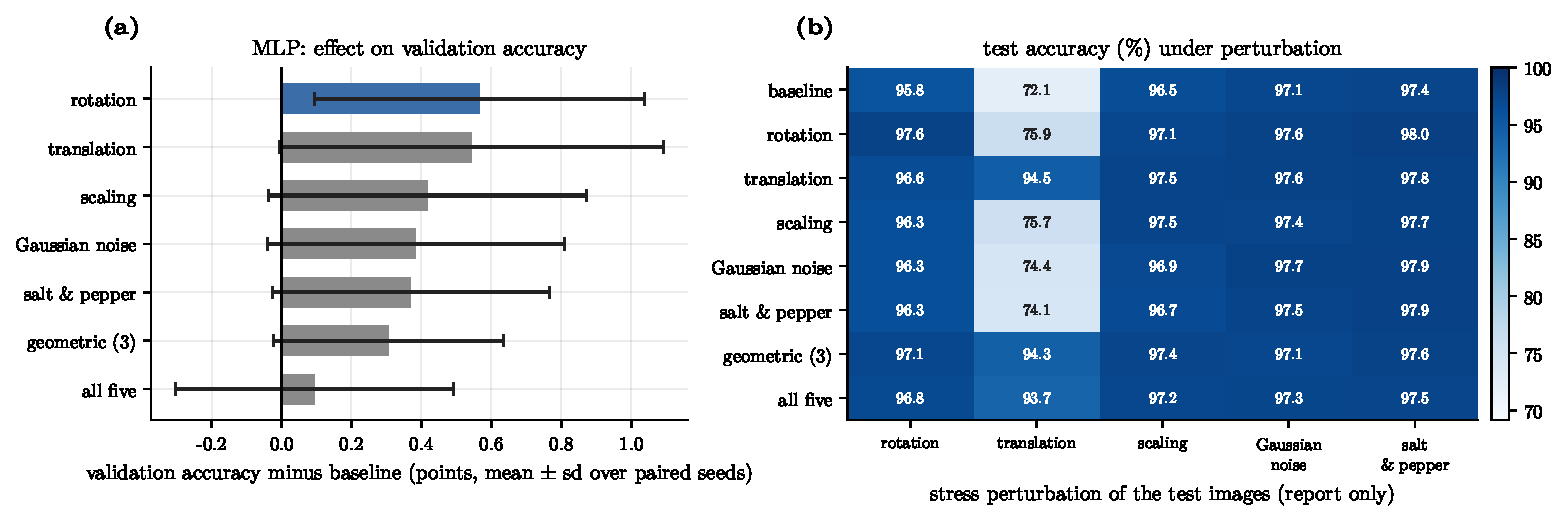
\includegraphics[width=\textwidth]{../results/figures/augmentation_mlp.pdf}
\caption{MLP: (a) hiệu validation accuracy so với điều kiện gốc (trung bình $\pm$ độ lệch chuẩn của hiệu ghép cặp); (b) accuracy trên ảnh test bị biến đổi mạnh.}
\label{fig:aug-mlp}
\end{figure}

\textbf{Đọc kết quả MLP.} Trên ảnh sạch, mọi điều kiện cho validation accuracy cao hơn điều kiện gốc nhưng hiệu ghép cặp có độ lệch chuẩn cùng bậc với chính mức tăng, nên với số seed hiện có chúng tôi \emph{không} khẳng định phép biến đổi nào cải thiện độ chính xác trên ảnh sạch; một phần mức tăng có thể đến từ việc có gấp đôi dữ liệu. Ngược lại, tác dụng \emph{đúng loại} lên độ bền rất rõ: huấn luyện với phép dịch nâng accuracy trên ảnh bị dịch mạnh lên rất nhiều so với điều kiện gốc, huấn luyện với xoay giúp trên ảnh bị xoay, và nhiễu nhẹ giúp ít vì MLP vốn đã khá bền với nhiễu. Cả năm phép cùng lúc không tốt hơn các phép riêng lẻ ở thí nghiệm này, tức là ``thêm mọi thứ'' không phải lúc nào cũng có lợi. Điều kiện có validation cao nhất được chọn theo quy tắc đã nêu, và mức chênh với điều kiện đứng sau nằm trong độ nhiễu.

\IfFileExists{generated/augmentation_cnn.tex}{
\begin{table}[H]\centering\scriptsize
\setlength{\tabcolsep}{3pt}
\begin{tabular}{lrrrrrrrrr}
\toprule
 & & \multicolumn{2}{c}{Validation} & Test & \multicolumn{5}{c}{Test sau nhiễu (\%)} \\
\cmidrule(lr){3-4}\cmidrule(lr){6-10}
Điều kiện & Số mẫu & Acc (\%) & $\Delta$ so với gốc & Acc (\%) & Xoay & Dịch & Co giãn & Gauss & Muối tiêu \\
\midrule
Không tăng cường & 50\,000 & 98.67 $\pm$ 0.04 & +0.00 $\pm$ 0.00 & 98.82 & 97.5 & 88.4 & 98.4 & 97.2 & 97.5 \\
Xoay & 100\,000 & 98.91 $\pm$ 0.05 & +0.23 $\pm$ 0.01 & 99.17 & 98.6 & 90.4 & 98.8 & 97.8 & 97.0 \\
Dịch chuyển & 100\,000 & 98.89 $\pm$ 0.06 & +0.22 $\pm$ 0.03 & 99.17 & 98.0 & 97.0 & 99.0 & 95.0 & 96.0 \\
Co giãn & 100\,000 & 98.87 $\pm$ 0.03 & +0.20 $\pm$ 0.01 & 99.06 & 97.7 & 90.5 & 98.8 & 97.4 & 97.0 \\
Nhiễu Gauss & 100\,000 & 98.87 $\pm$ 0.16 & +0.19 $\pm$ 0.20 & 99.06 & 97.7 & 90.2 & 98.8 & 98.3 & 97.8 \\
Nhiễu muối tiêu & 100\,000 & 98.84 $\pm$ 0.02 & +0.17 $\pm$ 0.06 & 99.00 & 97.8 & 89.8 & 98.6 & 98.4 & 98.7 \\
Hình học (xoay, dịch, co giãn) & 100\,000 & 98.92 $\pm$ 0.19 & +0.25 $\pm$ 0.16 & 99.20 & 98.5 & 97.2 & 98.9 & 93.6 & 95.0 \\
Cả năm phép & 100\,000 & 98.99 $\pm$ 0.03 & +0.31 $\pm$ 0.01 & 99.25 & 98.5 & 96.9 & 99.0 & 98.9 & 98.9 \\
\bottomrule
\end{tabular}
\caption{CNN với cấu hình đã chọn, huấn luyện lại với 2 seed (42, 43) cho mỗi điều kiện; $\Delta$ là hiệu validation accuracy so với điều kiện gốc \emph{cùng seed} (trung bình $\pm$ độ lệch chuẩn mẫu). 1 bản sao biến đổi cho mỗi ảnh train; điều kiện được chọn chỉ theo validation (\texttt{all}). Các cột ``Test sau nhiễu'' đo độ bền trên tập test bị biến đổi ở mức mạnh hơn mức huấn luyện, chỉ để báo cáo.}
\label{tab:augmentation-cnn}
\end{table}

\begin{figure}[H]\centering
\IfFileExists{../results/figures/augmentation_cnn.pdf}{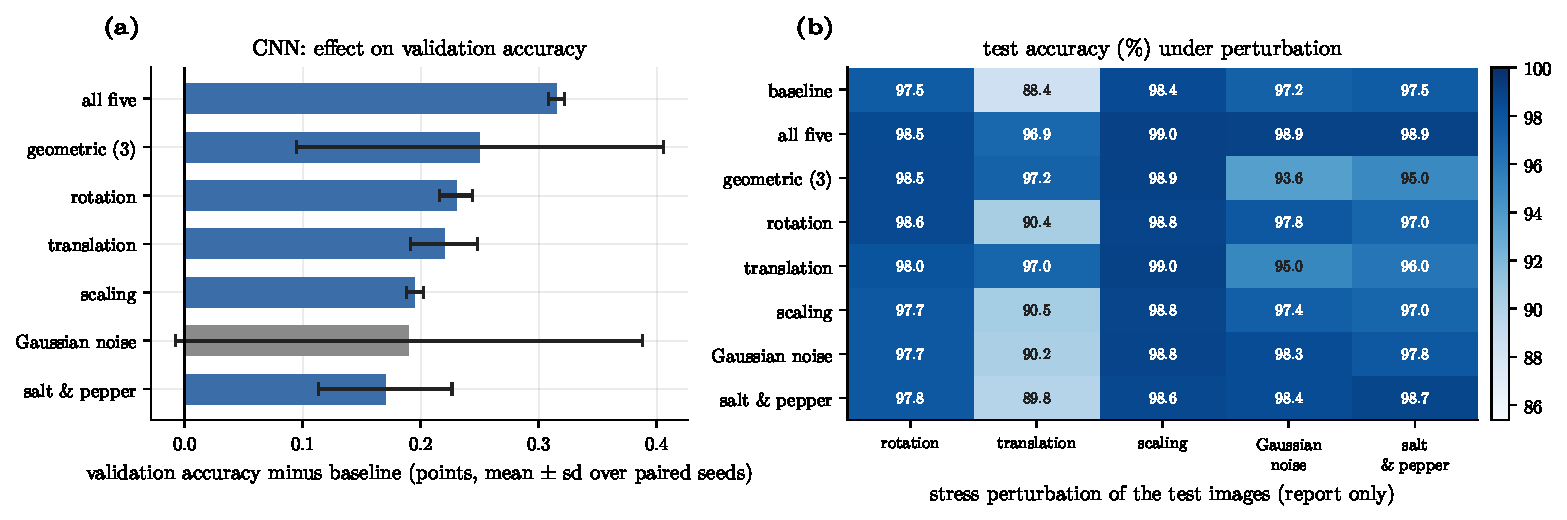
\includegraphics[width=\textwidth]{../results/figures/augmentation_cnn.pdf}}{}
\caption{CNN: cùng bố trí như Hình~\ref{fig:aug-mlp}.}
\label{fig:aug-cnn}
\end{figure}}{}

\textbf{Đọc kết quả CNN.} Với CNN, mọi điều kiện đều có validation accuracy cao hơn điều kiện gốc với hiệu ghép cặp ($+0.17$ \ldots{} $+0.31$ điểm, tuỳ điều kiện) lớn hơn độ lệch chuẩn của chúng ở hầu hết điều kiện, và ``cả năm phép'' có validation cao nhất nên được chọn theo quy tắc. Tuy nhiên chỉ có \emph{hai seed}, độ lệch chuẩn ước lượng từ hai giá trị kém tin cậy, và vẫn có yếu tố trộn lẫn là dữ liệu gấp đôi; vì vậy đây là bằng chứng gợi ý chứ chưa chắc chắn. Có một tác dụng \emph{bất lợi} rõ ràng: huấn luyện chỉ với phép dịch hoặc với nhóm hình học làm CNN \emph{kém bền hơn} với nhiễu Gauss và muối tiêu so với điều kiện gốc (ví dụ trên ảnh bị nhiễu Gauss mạnh, accuracy là $97.2\%$ ở điều kiện gốc nhưng chỉ $95.0\%$ khi huấn luyện với phép dịch và $93.6\%$ với nhóm hình học), trong khi huấn luyện với chính loại nhiễu đó hoặc với cả năm phép thì cải thiện. Tức là một phép tăng cường có thể cải thiện loại biến đổi nó mô phỏng và làm giảm độ bền ở loại khác; chỉ ``cả năm phép'' tốt đồng thời ở mọi cột cho CNN, còn với MLP thì không.

\subsection{CNN nhỏ so với MLP}
\label{sec:cnn}
Cấu hình CNN (Mục~\ref{sec:cnn-method}) được chọn bằng quét tuần tự trên validation như các mô hình khác (kênh, kích thước kernel, lớp dày đặc, tốc độ học, batch, dropout); toàn bộ nhật ký nằm trong \texttt{results/tuning/}. Bảng~\ref{tab:cnn-vs-mlp} và Hình~\ref{fig:cnn-vs-mlp} so sánh hai mô hình trên cùng $10\,000$ ảnh test.

\begin{table}[H]\centering\small
\begin{tabular}{lrr}
\toprule
 & MLP & CNN \\
\midrule
Số tham số & 535\,818 & 56\,714 \\
Kích thước ONNX (KiB) & 2094 & 223 \\
Accuracy test (\%) & 98.24 & 98.80 \\
Precision / Recall / F1 macro (\%) & 98.23 / 98.23 / 98.23 & 98.79 / 98.79 / 98.79 \\
Accuracy train $-$ test (điểm) & 1.63 & 0.60 \\
Thời gian huấn luyện (s) & 11 & 143 \\
Độ trễ một ảnh (ms) & 0.042 & 0.315 \\
Accuracy khi xoay (\%) & 96.00 & 97.46 \\
Accuracy khi dịch (\%) & 72.86 & 88.14 \\
Accuracy khi co giãn (\%) & 96.71 & 98.48 \\
Accuracy khi nhiễu Gauss (\%) & 97.31 & 98.07 \\
Accuracy khi muối tiêu (\%) & 97.56 & 97.71 \\
\bottomrule
\end{tabular}
\caption{CNN và MLP trên MNIST, cùng giao thức; mọi số lấy từ các lần chạy đã ghi. Hàng cuối: ảnh test bị biến đổi cố định (seed 999, mức mạnh hơn lúc huấn luyện), chỉ để báo cáo. Kiểm định McNemar chính xác trên dự đoán test: chỉ MLP đúng 64 ảnh, chỉ CNN đúng 120 ảnh, $p=4.4e-05$.}
\label{tab:cnn-vs-mlp}
\end{table}

\begin{figure}[H]\centering
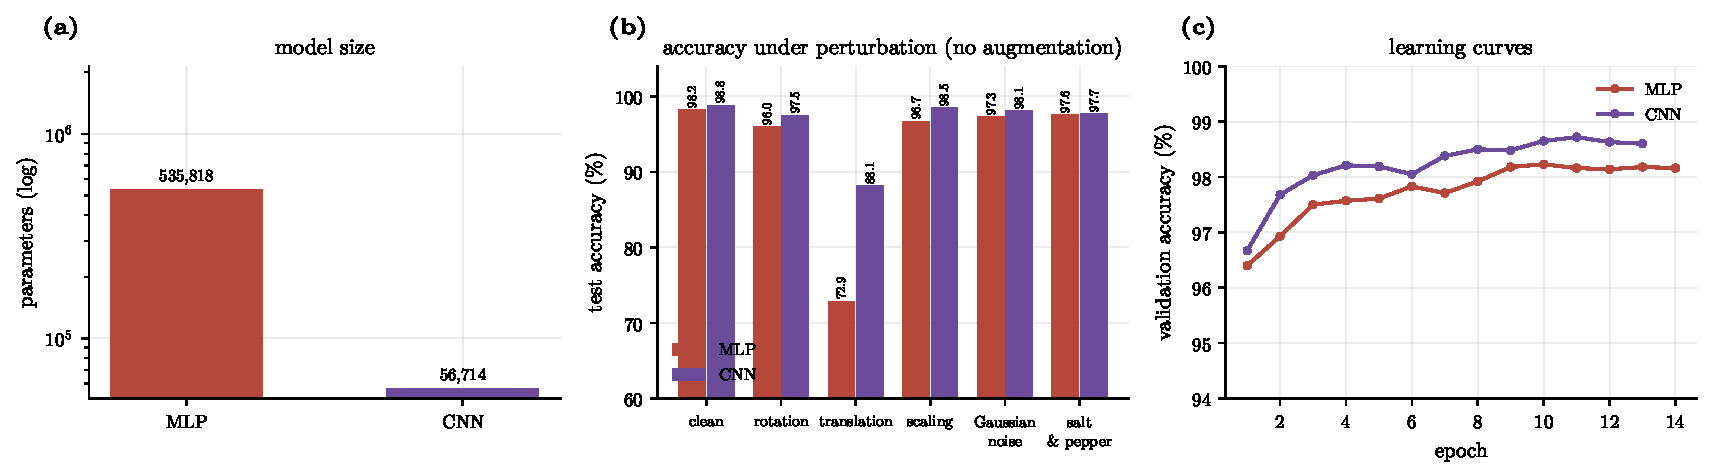
\includegraphics[width=\textwidth]{../results/figures/cnn_vs_mlp.pdf}
\caption{CNN và MLP: số tham số, độ bền khi ảnh test bị biến đổi (không dùng tăng cường), đường cong validation.}
\label{fig:cnn-vs-mlp}
\end{figure}

CNN có accuracy cao hơn MLP (\accTestCNN\% so với \accTestMLP\%) và khác biệt này có ý nghĩa thống kê trên cùng ảnh test (McNemar chính xác, Bảng~\ref{tab:cnn-vs-mlp}), với \emph{khoảng một phần mười} số tham số, khoảng cách train--test nhỏ hơn và bền hơn rõ rệt khi ảnh bị dịch -- đúng điều ta mong đợi từ chia sẻ trọng số và gộp cục bộ. Cái giá là thời gian huấn luyện (\fitCNN\,s so với \fitMLP\,s) và độ trễ mỗi ảnh (\latCNN\,ms so với \latMLP\,ms) cao hơn. Về diễn giải, nơ-ron lớp đầu của MLP có một trọng số cho mỗi pixel nên vẽ được thành ảnh $28\times28$, còn kernel $3\times3$ của CNN dùng chung ở mọi vị trí nên dễ vẽ (Hình~\ref{fig:cnn-filters}) nhưng một kernel riêng lẻ nói rất ít về quyết định cuối cùng nếu không xét các tầng sau; đây là nhận xét định tính, không phải một điểm số đo được.

\begin{figure}[H]\centering
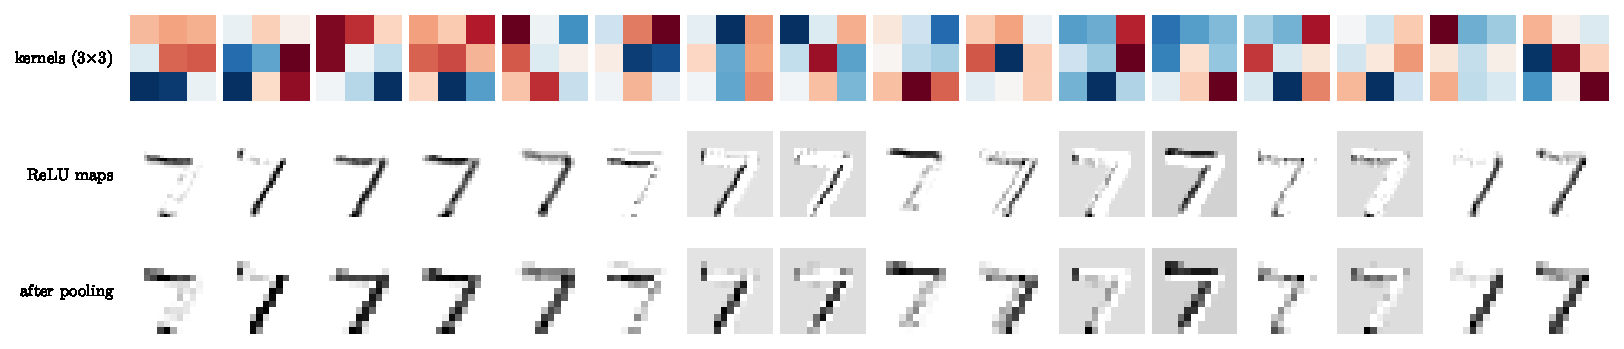
\includegraphics[width=0.85\textwidth]{../results/figures/cnn_filters.pdf}
\caption{Kernel $3\times3$ lớp đầu đã học, bản đồ ReLU và kết quả sau gộp cho một ảnh test thật. Bản đồ kích hoạt cho thấy lớp \emph{tính ra gì}, không chứng minh vùng nào gây ra quyết định.}
\label{fig:cnn-filters}
\end{figure}

\subsection{Trình khám phá thực thi mô hình trên trình duyệt}
\label{sec:explorer}
Mục ``nhìn vào bên trong'' của trang web được làm lại thành một trình khám phá chỉ vẽ những gì \emph{mô hình đang triển khai} thực sự tính, không có mạng giả, kích hoạt giả hay kiến trúc gõ cứng trong giao diện.

\textbf{Dòng thông tin.} (1) Python sinh \emph{hợp đồng vết} \texttt{writerhand.trace/1} từ chính đối tượng mô hình đã huấn luyện (\texttt{src/export/tracespec.py}): định danh mô hình, đồ thị lớp (DAG với toán tử, đầu vào, hình dạng đầu ra), tiền xử lý, bảng tham số (vị trí trong \texttt{params.bin}, hình dạng, mã băm), danh sách đầu ra trung gian cần lấy từ đồ thị, loại đầu ra (xác suất softmax hay tỉ lệ phiếu \emph{chưa hiệu chỉnh}). (2) Bundle gồm manifest (có \texttt{bundle\_id} và SHA-256 từng tệp), ONNX, \texttt{params.bin}, ensemble AdaBoost nhị phân, ảnh test mẫu cùng đầu ra kỳ vọng và bản ghi huấn luyện; nó được đẩy lên Hugging Face và \emph{ghim theo mã commit} trong \texttt{web/model-lock.json}; trang web chỉ tải đúng revision đó, kiểm tra SHA-256 manifest so với bản đã commit cùng trang, và kiểm tra từng tệp. (3) Trình duyệt kiểm tra hợp đồng, chạy ONNX Runtime Web với đúng các đầu ra mà hợp đồng khai báo, rồi vẽ sơ đồ \emph{từ metadata}: đổi kiến trúc rồi huấn luyện lại thì sơ đồ tự đổi. (4) Mỗi kết quả thực thi mang dấu (bundle, bộ dữ liệu, mô hình, dấu vân tay của ảnh) và bị loại bỏ khi bất kỳ yếu tố nào đổi, nên không bao giờ hiển thị kết quả cũ.

\textbf{Từng mô hình.} \emph{MLP}: $28\times28\to$ duỗi phẳng $784\to$ chuẩn hóa $\to$ các lớp dày đặc với nơ-ron/kết nối chọn được; một tổng có trọng số được tái dựng từ tham số và đặt cạnh giá trị của đồ thị kèm sai lệch tuyệt đối; lớp lớn được rút gọn bằng cách hiển thị các số hạng lớn nhất và ghi rõ đã rút gọn. \emph{CNN}: kernel, bản đồ đặc trưng, cửa sổ trượt với phép nhân--cộng từng pixel, ReLU, cửa sổ gộp và giá trị cực đại, trường tiếp nhận, hình dạng từng tầng và điểm số. \emph{Naïve Bayes}: trung bình, phương sai, số hạng log-likelihood theo lớp và pixel, tổng cộng dồn đối chiếu với log joint của đồ thị. \emph{Softmax}: $x_iW_{ik}$, bias, cộng dồn và đối chiếu với logit. \emph{AdaBoost-SAMME}: các cây thật (pixel, ngưỡng, nhánh, lớp ở lá), $\alpha_t$, phiếu cộng dồn có thể tạm dừng, bước và kéo; các giá trị này là \emph{tỉ lệ phiếu có trọng số}, không phải xác suất đã hiệu chỉnh. Mọi phép phát có Play/Pause/Step/Back/Replay, tốc độ, chế độ giảm chuyển động và cho xem giá trị không cần dừng.

\textbf{Hai chế độ tách biệt.} \emph{Suy luận} trên ảnh người dùng, và \emph{phát lại huấn luyện} chỉ từ các điểm kiểm tra và số đo \emph{thật} đã ghi lúc huấn luyện lại với đúng cấu hình và seed (\texttt{writerhand.replay/1}): mất mát và độ chính xác theo epoch, dự đoán của chính mô hình trên $12$ ảnh train cố định ở các epoch được chọn, và một phần trọng số (softmax: toàn bộ $W$; MLP: $16$ nơ-ron đầu của lớp thứ nhất; CNN: mọi kernel). Tệp ghi epoch mà mô hình triển khai tương ứng (\texttt{deployed\_epoch}, do dừng sớm khôi phục trọng số tốt nhất) và chỉ đánh dấu khớp khi trọng số đã lưu bằng đúng trọng số triển khai. Naïve Bayes không có huấn luyện lặp nên không có phát lại; AdaBoost dùng các tiền tố của chính ensemble đã triển khai.

\subsection{Trực quan hóa tính toán không phải giải thích quyết định}
\label{sec:viz-vs-explain}
Một bản đồ kích hoạt, một kernel hay một đường đi trong cây cho biết mô hình \emph{đã tính gì} với ảnh này; nó không chứng minh rằng điểm ảnh hay bộ lọc đó \emph{gây ra} quyết định, vì các tầng sau có thể bù trừ hoặc bỏ qua. Trong trình khám phá, chỉ những phân rã \emph{chính xác theo cấu trúc mô hình} (số hạng $x_iW_{ik}$ của softmax, đóng góp log-likelihood của Naïve Bayes, phiếu của từng cây) được gọi là phần đóng góp vào điểm số, và vẫn không được gọi là ``lý do'' theo nghĩa nhân quả; các kích hoạt của MLP/CNN được ghi nhãn là giá trị trung gian. Chúng tôi không dùng phương pháp quy gán (Grad-CAM, tích phân gradient, \ldots) và không tuyên bố rằng chúng được kiểm chứng.

\subsection{Theo dõi thí nghiệm và công cụ tìm siêu tham số}
Siêu tham số được tìm bằng \emph{quét tuần tự từng tham số} (coordinate descent) do nhóm tự viết (\texttt{src/experiments/search.py}), không dùng Optuna hay thư viện tối ưu siêu tham số: chi phí là tổng số giá trị thay vì tích, và mỗi lượt quét chính là đồ thị ``đổi một siêu tham số, giữ nguyên phần còn lại''. Nhược điểm là không xét tương tác giữa các siêu tham số. Mọi lần chạy được ghi bằng Weights \& Biases ở chế độ \emph{offline} (máy nhóm chưa có khóa API; có thể \texttt{wandb sync} sau), bên cạnh nhật ký JSON luôn được ghi trong \texttt{results/}.

\subsection{Bản demo web và quy trình triển khai}
\label{sec:demo}
Mô hình được xuất ra một bundle gồm ONNX cho Naïve Bayes, softmax, MLP và CNN (đồ thị dựng tay bằng \texttt{onnx.helper}, bước chuẩn hóa $(x-\bar x)/(s+\varepsilon)$ nằm \emph{trong} đồ thị nên tiền xử lý huấn luyện và suy luận trùng nhau) và một tệp nhị phân cho các cây của AdaBoost (bộ đánh giá viết bằng TypeScript). Mỗi tệp xuất được kiểm tra số học trên toàn bộ ảnh test của bộ dữ liệu tương ứng: Gaussian NB: sai lệch xác suất lớn nhất $1.4e-04$\, trùng nhãn 100.00\% trên 2\,000 ảnh; Softmax regression: sai lệch xác suất lớn nhất $3.4e-06$\, trùng nhãn 100.00\% trên 2\,000 ảnh; MLP: sai lệch xác suất lớn nhất $1.7e-06$\, trùng nhãn 100.00\% trên 2\,000 ảnh; AdaBoost-SAMME: sai lệch xác suất lớn nhất $0.0e+00$\, trùng nhãn 100.00\% trên 2\,000 ảnh; CNN: sai lệch xác suất lớn nhất $7.2e-07$\, trùng nhãn 100.00\% trên 2\,000 ảnh%
. Bundle cùng model card được đẩy lên Hugging Face Hub (\url{https://huggingface.co/TranTrinhNhan1111/WriteRHand-MNIST}; không đưa trọng số lên GitHub), và trang demo được triển khai trên GitHub Pages (\url{https://trantrinhnhan1.github.io/WriteRHand/}). Trang web (React + TypeScript + Vite + ONNX Runtime Web, hoàn toàn tĩnh) cho phép vẽ hoặc tải ảnh, chọn bộ dữ liệu và một trong năm mô hình (chỉ những mô hình có tệp đã kiểm chứng), xem ảnh $28\times28$ sau tiền xử lý, top-$k$, bảng kết quả, ma trận nhầm lẫn và đường cong; ảnh vẽ được cắt, thu về hộp $20\times20$ và căn trọng tâm về $(14,14)$ đúng như quy trình tạo MNIST. Quy trình CI (GitHub Actions) chạy kiểm tra mã, kiểm thử đơn vị, một lượt chạy thử nhỏ của pipeline, kiểm tra manifest--khóa--revision từ xa khớp nhau, kiểm thử trình duyệt trên bundle đã ghim và build giao diện; không huấn luyện lại ở mỗi commit. Mô hình cho bản demo và các bảng chính vẫn là các mô hình huấn luyện trên dữ liệu gốc (không tăng cường).
